
\begin{figure}[!h]
\centering
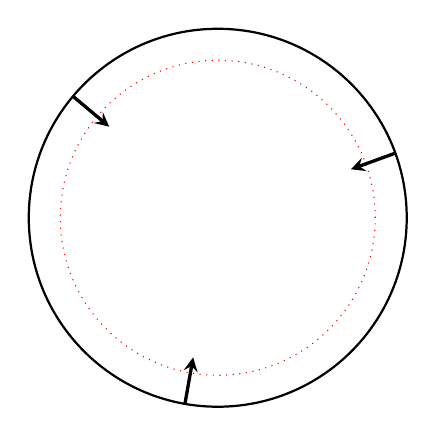
\begin{tikzpicture}[scale=2,>=stealth]
%Draw Circle radius 1 cm
    \draw[black,thick] (0,0) circle (1.2cm);
    \draw[red,dotted] (0,0) circle (1cm);
     \foreach \angle/\count in {20/1,140/2,260/3}
        {

%Draws the 3 acceleration vectors directed inward and offset slightly from the distance vectors
        \draw [name=acceleration vectors,very thick,->]
            (\angle:1.2cm) -- node[midway] {} (\angle:0.9cm) ;
    }
\end{tikzpicture}
\end{figure}



\begin{figure}[!h]
\centering
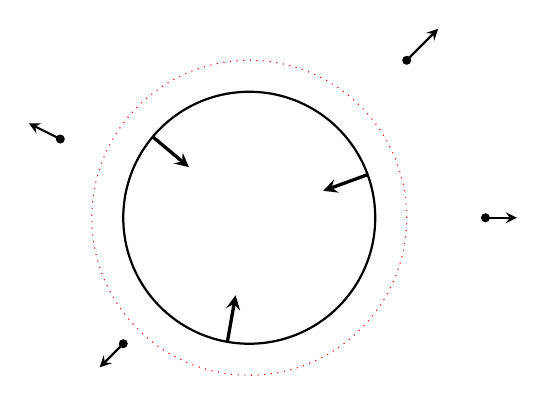
\begin{tikzpicture}[scale=2,>=stealth]
%Draw Circle radius 1 cm
    \draw[black,thick] (0,0) circle (0.8cm);
    \draw[red,dotted] (0,0) circle (1cm);
     \foreach \angle/\count in {20/1,140/2,260/3}
        {

%Draws the 3 acceleration vectors directed inward and offset slightly from the distance vectors
        \draw [name=acceleration vectors,very thick,->]
            (\angle:0.8cm) -- node[midway] {} (\angle:0.5cm) ;
    }
    \node[draw,circle,inner sep=1pt,fill] at (1,1)[] {};
    \node[draw,circle,inner sep=1pt,fill] at (1.5,0)[] {};
    \node[draw,circle,inner sep=1pt,fill] at (-1.2,0.5)[] {};
    \node[draw,circle,inner sep=1pt,fill] at (-0.8,-0.8)[] {};
    \draw [->,thick](1,1) -- (1.2,1.2);
    \draw [->,thick](1.5,0) -- (1.7,0);
    \draw [->,thick](-1.2,0.5) -- (-1.4,0.6);
    \draw [->,thick](-0.8,-0.8) -- (-0.95,-0.95);
\end{tikzpicture}
\end{figure}



\begin{figure}[!h]
\centering
\begin{tikzpicture}[scale=2,>=stealth]
%Draw Circle radius 1 cm
    \draw[black,thick] (0,0) circle (0.4cm);
    \draw[red,dotted] (0,0) circle (0.6cm);
     \foreach \angle/\count in {20/1,140/2,260/3}
        {

%Draws the 3 acceleration vectors directed inward and offset slightly from the distance vectors
        \draw [name=acceleration vectors,very thick,->]
            (\angle:0.4cm) -- node[midway] {} (\angle:0.2cm) ;
    }
    \node[draw,circle,inner sep=1pt,fill] at (1,1)[] {};
    \node[draw,circle,inner sep=1pt,fill] at (1.5,0)[] {};
    \node[draw,circle,inner sep=1pt,fill] at (-1.2,0.5)[] {};
    \node[draw,circle,inner sep=1pt,fill] at (-0.8,-0.8)[] {};
    \node[draw,circle,inner sep=1pt,fill] at (0,0.88)[] {};
    \node[draw,circle,inner sep=1pt,fill] at (0.6,-0.48)[] {};
    \draw [->,thick](1,1) -- (1.2,1.2);
    \draw [->,thick](1.5,0) -- (1.7,0);
    \draw [->,thick](-1.2,0.5) -- (-1.4,0.6);
    \draw [->,thick](-0.8,-0.8) -- (-0.95,-0.95);
    \draw [->,thick](0,0.88) -- (0,1.1);
    \draw [->,thick](0.6,-0.48) -- (0.7,-0.7);
\end{tikzpicture}
\end{figure}




\begin{figure}[!h]
\centering
\begin{tikzpicture}[scale=2,>=stealth]
%Draw Circle radius 1 cm
  
    \node[draw,circle,inner sep=1pt,fill] at (1,1)[] {};
    \node[draw,circle,inner sep=1pt,fill] at (1.5,0)[] {};
    \node[draw,circle,inner sep=1pt,fill] at (-1.2,0.5)[] {};
    \node[draw,circle,inner sep=1pt,fill] at (-0.8,-0.8)[] {};
    \node[draw,circle,inner sep=1pt,fill] at (0,0.88)[] {};
    \node[draw,circle,inner sep=1pt,fill] at (0.6,-0.48)[] {};
    \draw [->,thick](1,1) -- (1.2,1.2);
    \draw [->,thick](1.5,0) -- (1.7,0);
    \draw [->,thick](-1.2,0.5) -- (-1.4,0.6);
    \draw [->,thick](-0.8,-0.8) -- (-0.95,-0.95);
    \draw [->,thick](0,0.88) -- (0,1.1);
    \draw [->,thick](0.6,-0.48) -- (0.7,-0.7);
    
    \node[draw=none] at (0,0) {Poof!};
\end{tikzpicture}
\end{figure}

